% Asset ID: AS2CorrelationAndRegressionLinesTikZ-005
% Source: CCEA AS2-DPI-LO007 + S1-Chp4-Correlation.pdf page 6
% Related section: Core Theory - Correlation does not imply causation
% Purpose: Show association, invalid causal leap and possible lurking variable.
\documentclass[tikz,border=6pt]{standalone}
\usepackage{amsmath}
\usetikzlibrary{arrows.meta,positioning}
\begin{document}
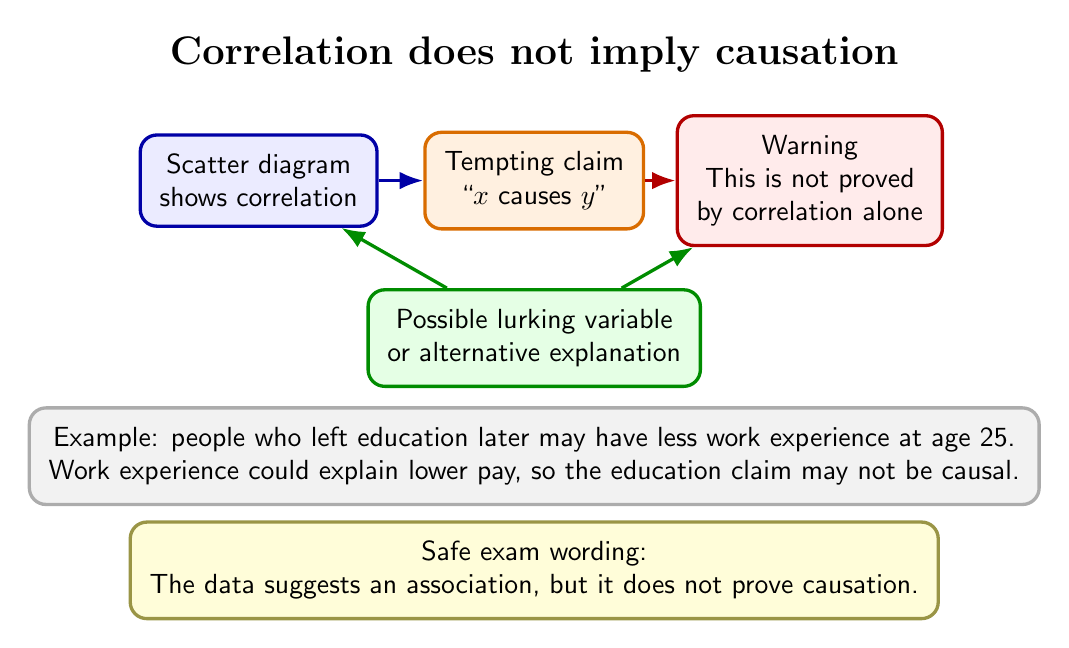
\begin{tikzpicture}[font=\sffamily,>={Latex[length=3mm]},box/.style={draw, rounded corners=6pt, very thick, align=center, inner sep=7pt},arrow/.style={->, very thick}]
\node[font=\bfseries\Large] at (5.5,5.9) {Correlation does not imply causation};
\node[box, fill=blue!8, draw=blue!65!black] (corr) at (2.0,4.3) {Scatter diagram\\shows correlation};
\node[box, fill=orange!12, draw=orange!85!black] (claim) at (5.5,4.3) {Tempting claim\\``$x$ causes $y$''};
\node[box, fill=red!8, draw=red!70!black] (warn) at (9.0,4.3) {Warning\\This is not proved\\by correlation alone};
\draw[arrow, blue!65!black] (corr) -- (claim);\draw[arrow, red!70!black] (claim) -- (warn);
\node[box, fill=green!10, draw=green!55!black] (third) at (5.5,2.3) {Possible lurking variable\\or alternative explanation};
\draw[arrow, green!55!black] (third) -- (corr);\draw[arrow, green!55!black] (third) -- (warn);
\node[box, fill=gray!10, draw=gray!65] at (5.5,0.8) {Example: people who left education later may have less work experience at age 25.\\Work experience could explain lower pay, so the education claim may not be causal.};
\node[box, fill=yellow!15, draw=yellow!55!black] at (5.5,-0.65) {Safe exam wording:\\The data suggests an association, but it does not prove causation.};
\end{tikzpicture}\end{document}
